\subsection{Bài toán lát sàn nhà}

Trong xã hội hiện đại ngày nay, đi đâu cũng có thể nhìn thấy những viên gạch lát sàn nhà. Dù muôn hình vạn trạng, tất cả các phép lát này (ta chỉ tính những phép lát đối xứng) đều chỉ là một trong 17 loại, nằm trong 17 "nhóm lát nền" (tạm dịch từ \textit{wallpaper group}).

Những nhóm này được xây dựng bằng các tập phép biến hình trên mặt phẳng, với phép toán hai ngôi là phép hợp. Chằng hạn nhóm $p0$ là nhóm chỉ gồm có các phép tịnh tiến, nhóm $p4m$, gồm có các hợp của các phép tịnh tiến, đối xứng gương và quay 90 độ.

\begin{figure}
\centering
\begin{subfigure}{.5\textwidth}
	\centering
	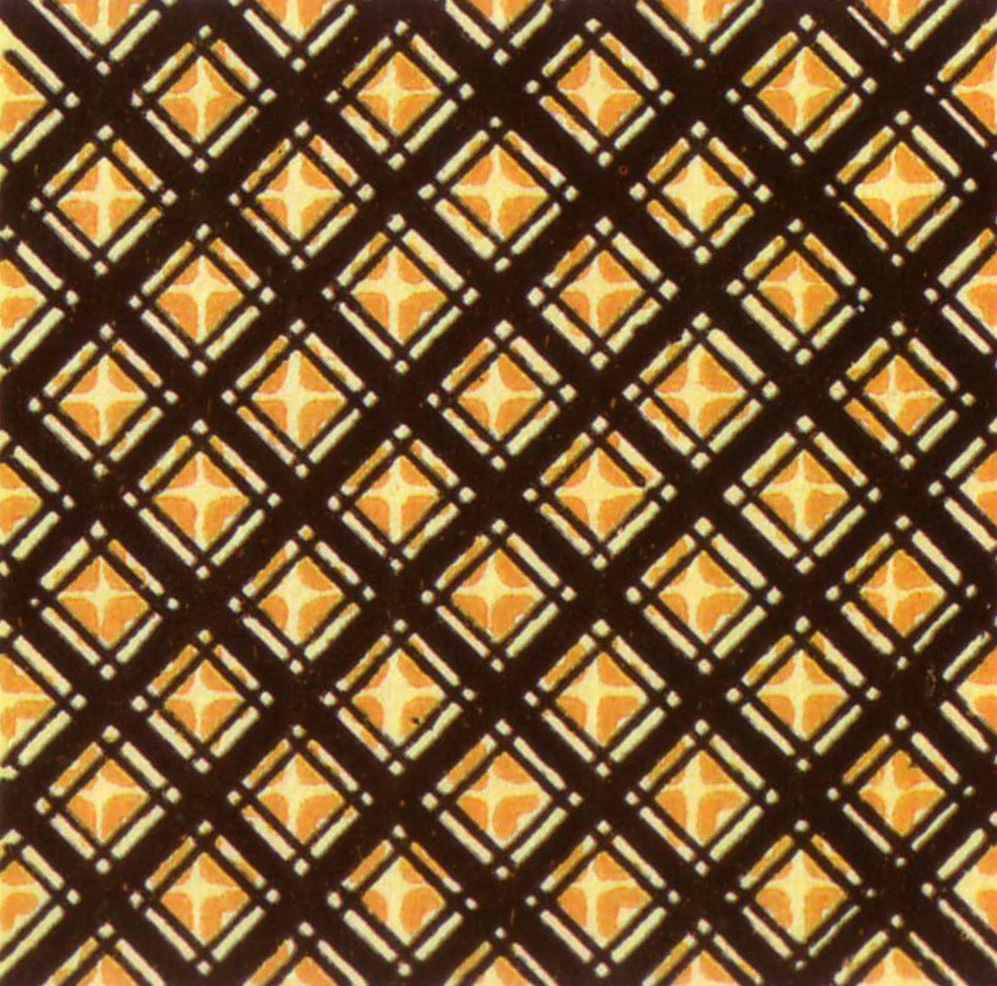
\includegraphics[width=.4\linewidth]{Wallpaper_group-p4m-2.jpg}
	\caption{Vải, Tahiti}
\end{subfigure}%
\begin{subfigure}{.5\textwidth}
	\centering
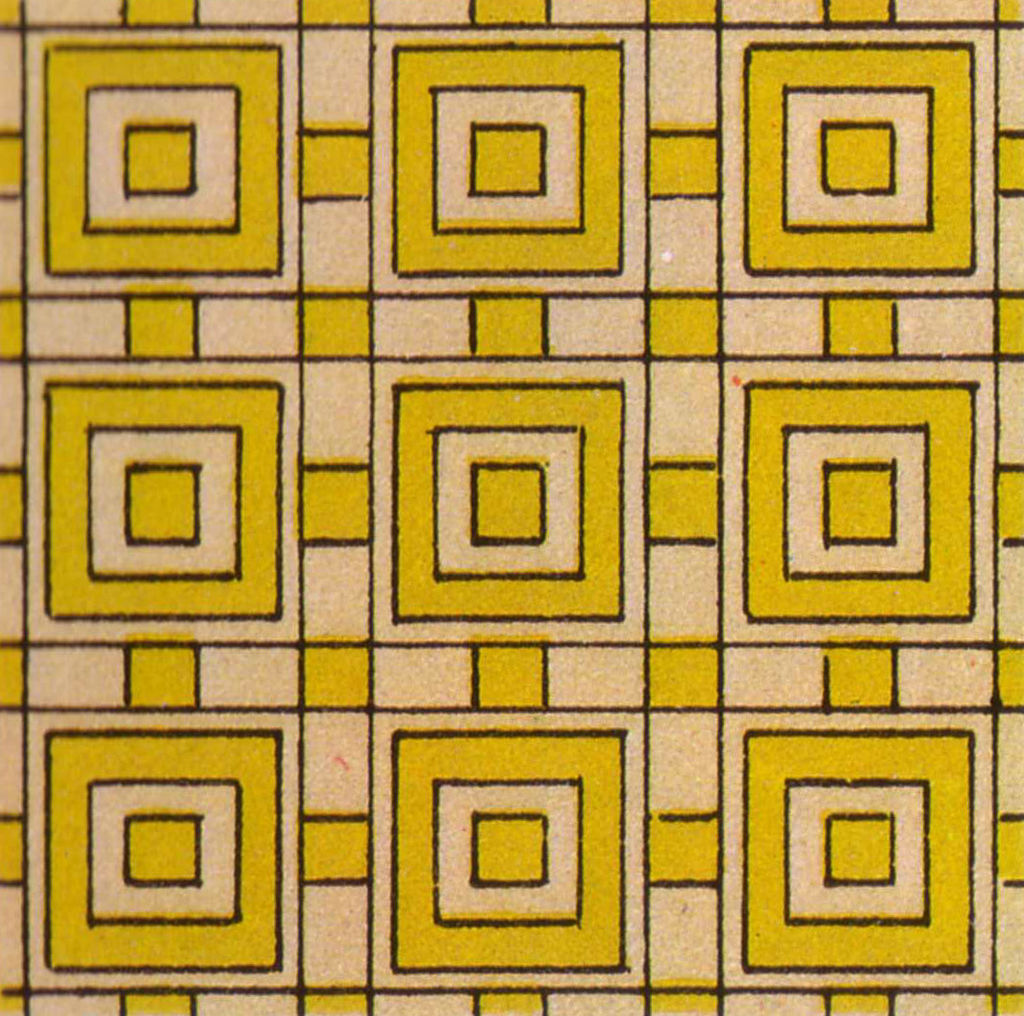
\includegraphics[width=.4\linewidth]{1024px-Wallpaper_group-p4m-1.jpg}
\caption{Tranh trang trí, Nineveh, Assyria}
\end{subfigure}%
	\caption{Hai cách lát cùng thuộc nhóm \textbf{p4m}}
\end{figure}

\subsection{Thuật toán nhân ma trận}

Trong thời đại hiện nay, làm việc với ma trận là một công việc quen thuộc của bất cứ chiếc máy tính hiện đại nào. Ứng dụng của những phép toán với ma trận có nhiều ứng dụng rộng rãi, trong các ứng dụng đồ họa 3D (bao gồm game) cũng như những hệ thống trí tuệ nhân tạo phức tạp. Trong đó, một phép toán được sử dụng nhiều chính là phép nhân ma trận. Chính vì thế, phép toán này trở thành một đề tài nghiên cứu vô cùng sôi nổi. 

Đa số các thuật toán nhân ma trận có độ phức tạp tính toán (computational complexity) thuộc dạng $O(n^\omega)$, với $\omega$ càng nhỏ, thuật toán càng nhanh (theo lý thuyết). Bạn đọc có thể dễ dàng chứng minh được rằng tồn tại một thuật toán với $\omega$ thỏa mãn $2 \le \omega \le 3$. Hiện tại, $\omega$ nhỏ nhất (tương đương với thuật toán nhanh nhất) là khoảng 2.37. 

Tuy nhiên, ứng dụng lý thuyết nhóm, Henry Cohn, Robert Kleinberg, Balázs Szegedy và Chris Umans đưa ra một một số phỏng đoán (conjecture), mà nếu đúng thì sẽ suy ra sự tồn tại của một thuật toán với $\omega$ bằng 2. Trong số các giả thuyết đó, một vài phỏng đoán đã bị chứng minh là không đúng.

\newpage
\begin{figure}
	\centering
	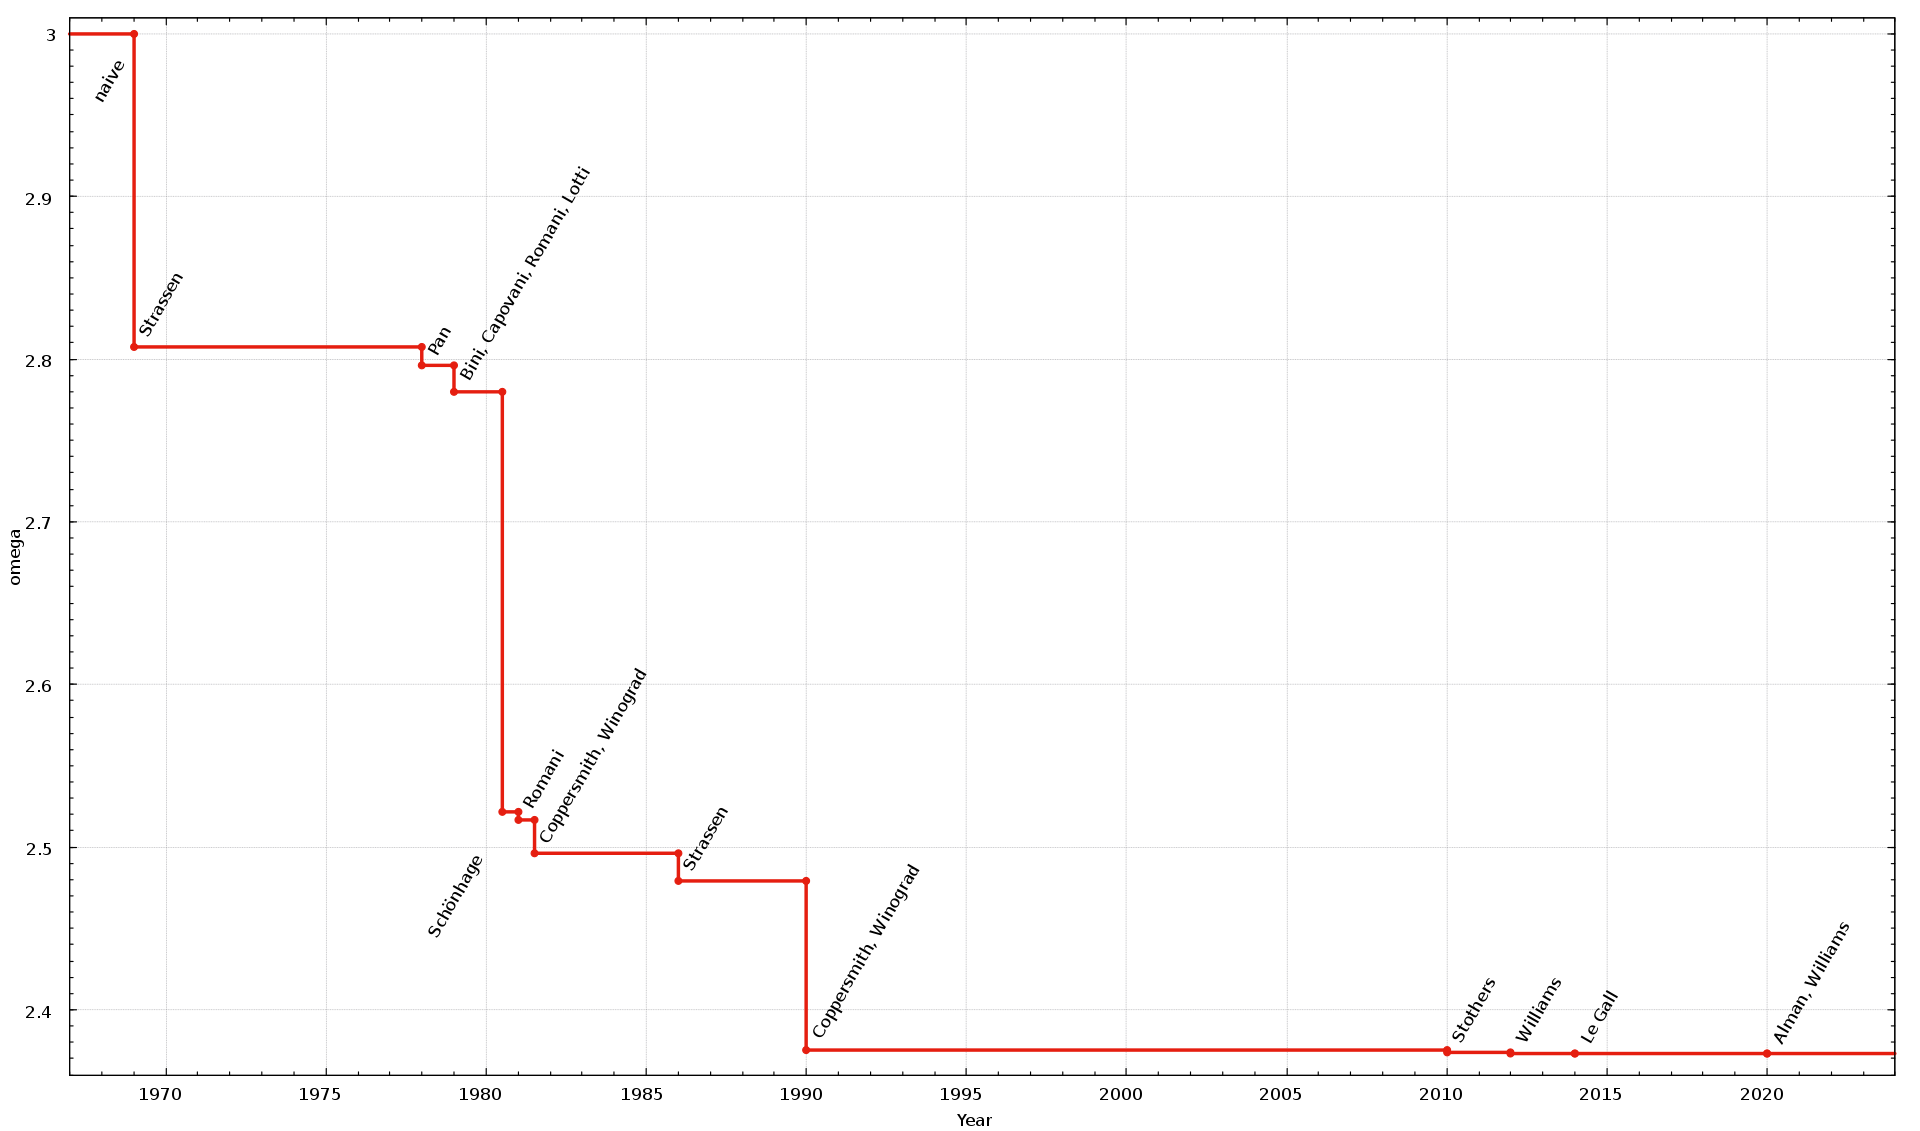
\includegraphics[width=.8\linewidth]{matrixmult.png}
	\caption{Quá trình tối ưu hóa thuật toán nhân ma trận (theo $\omega$) đến nay}
\end{figure}

\subsection{Các hành động lên một vật thể}

Ví dụ tiêu biểu nhất của ứng dụng này là trong việc xoay Rubik. Tổng quát nhất, có thể dễ thấy rằng tập các hành động có thể đảo ngược lên một vật thể (bao gồm hành động "không làm gì") cùng với phép "hợp" của các hành động là một nhóm.

Thật vậy, phép "hợp" này có tính chất kết hợp (bạn đọc có thể dễ dàng nhận ra điều này khi xoay một khối Rubik), có phần tử trung hòa/đơn vị là hành động "không làm gì", phần tử đối xứng với một hành động là hành động đảo ngược của hành động đó.

Ứng dụng này được sử dụng trong việc tạo ra thuật toán tối ưu cho giải Rubik, dù là 3x3 hay 1000x1000. 

Trong lý thuyết nhóm cũng có một khái niệm liên quan đến hiện tượng này, đó chính là hành động nhóm (group action).

\subsection{Sự đối xứng}

Lý thuyết nhóm được sử dụng nhiều trong việc nghiên cứu những cấu trúc đối xứng, như hạt nhân nguyên tử, các orbital trong hóa học, và mã hóa của các DNA.